\section{Backend}

\subsection{Tecnologies and libraries}

\subsubsection{NodeJs}
Node.js is an open-source, cross-platform, back-end JavaScript runtime environment that runs on the V8 engine and executes JavaScript code outside a web browser. Node.js lets developers use JavaScript to write command line tools and for server-side scripting—running scripts server-side to produce dynamic web page content before the page is sent to the user's web browser. Consequently, Node.js represents a "JavaScript everywhere" paradigm, unifying web-application development around a single programming language, rather than different languages for server-side and client-side scripts.

\begin{itemize}
    \item \textbf{Used Version:} 4.2.2 
\end{itemize}

\subsubsection{Typescript}
TypeScript is a programming language developed and maintained by Microsoft. It is a strict syntactical superset of JavaScript and adds optional static typing to the language. TypeScript is designed for the development of large applications and transcompiles to JavaScript. 
   
    \begin{itemize}
        \item \textbf{Used Version:} 4.2.2 
    \end{itemize}

\subsubsection{JSON}
JSON (JavaScript Object Notation) is an open standard file format, and data interchange format, that uses human-readable text to store and transmit data objects consisting of attribute–value pairs and array data types (or any other serializable value). It is a very common data format, with a diverse range of applications, such as serving as a replacement for XML in AJAX systems.


\subsubsection{DynamoDB}
Amazon DynamoDB is a fully managed proprietary NoSQL database service that supports key-value and document data structures and is offered by Amazon.com as part of the Amazon Web Services portfolio
\subsubsection{Npm}
npm is the package manager for the Node JavaScript platform. It puts modules in place so that node can find them, and manages dependency conflicts intelligently.
It is extremely configurable to support a wide variety of use cases. Most commonly, it is used to publish, discover, install, and develop node programs.
\subsubsection{Swagger}
Swagger is an Interface Description Language for describing RESTful APIs expressed using JSON. Swagger is used together with a set of open-source software tools to design, build, document, and use RESTful web services. Swagger includes automated documentation, code generation (into many programming languages), and test-case generation.


\subsection{Architecture}
We created a serverless and microservices oriented architecture. Each microservice is hosted in a different repository, with it's own persistence layer and CI rules.
The microservices created and their respective responsabilities are:
\begin{itemize}
    \item products: you can find the repo \href{https://github.com/SWException/products}{here}; it provides CRUD functionalities for products managment,
                    like create a new product, modify an existing one, etc... It has also the responsibiloty to manage images associated to a product, which are 
                    stored in a Amazon S3 bucket;
    \item carts: you can find the repo \href{https://github.com/SWException/carts}{here}; it has the responsibility to manage carts of all users and guests that
                 added some products to their carts. Carts are identified by the user ID (provided by Amazon Cognito), so it communicates with users microservice for each call.
                 Each cart contain only an array of tuples composed by a products ID and a quantity (integer);
    \item orders: you can find the repo \href{https://github.com/SWException/orders}{here}; it has the responsibility to provide CRUD functionalities for orders information.
                  It also has to provide API's to start and complete checkout process, communicating with Stripe to generate a payment intent;
    \item users: you can find the repo \href{https://github.com/SWException/users}{here}; it provide the functionality to check a Cognito's token JWT to other microservices.
                 It also provides to the frontend service the possibility to get the customers list and details about a specific customer;
    \item categories: you can find the repo \href{https://github.com/SWException/categories}{here}; it provides CRUD functionalities to manage categories information.
                      This is called, for example, each time that someone asks for product details to the products microservice;
    \item taxes: you can find the repo \href{https://github.com/SWException/taxes}{here}; it provides CRUD functionalities to manage taxes information;
    \item addresses: you can find the repo \href{https://github.com/SWException/addresses}{here}; it provides CRUD functionalities to manage addresses information.
\end{itemize}

\subsection{Class diagrams}
All services are projected with the same architectural pattern, each one has three layer:
\begin{itemize}
    \item the first contains one handler for each API defined in swagger;
    \item the second is the core and contains model logic;
    \item the third and last is the repository layer, which has the responability to interface the
          service with third part services, databases and other services of the backend module.
\end{itemize}
In the following paragraphs, we will present a class diagram for each service.

\subsubsection{Taxes service}
\begin{figure}[H]
    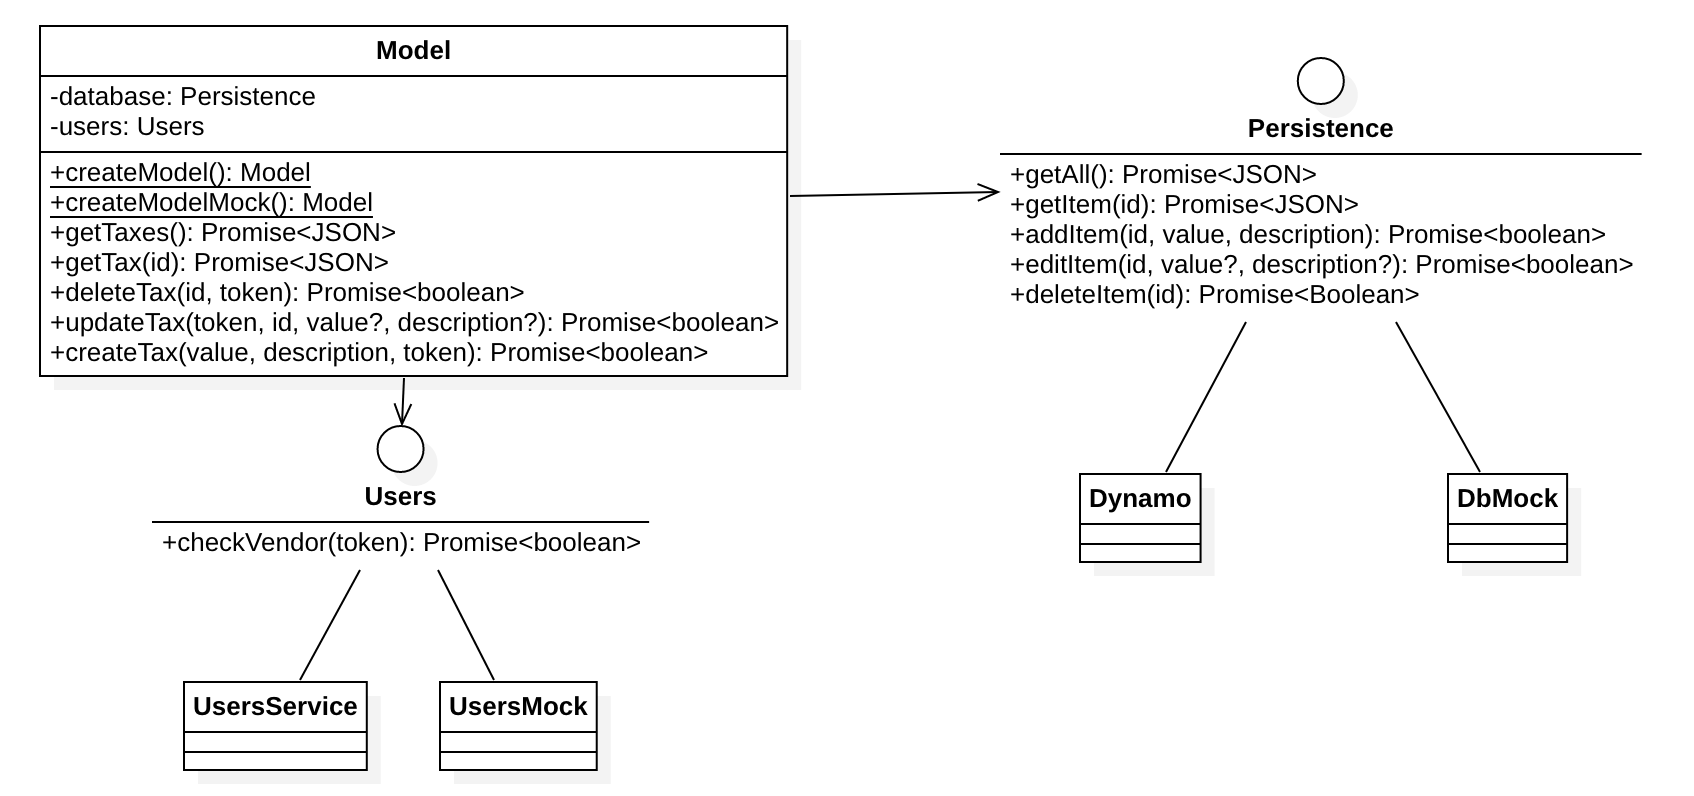
\includegraphics[width=0.9\textwidth]{res/images/class-diagrams/taxes.png}
\end{figure}

\subsubsection{Categories service}
\begin{figure}[H]
    
\includegraphics[width=0.9\textwidth]{res/images/class-diagrams/categories.png}
\end{figure}

\subsubsection{Orders service}
\begin{figure}[H]
    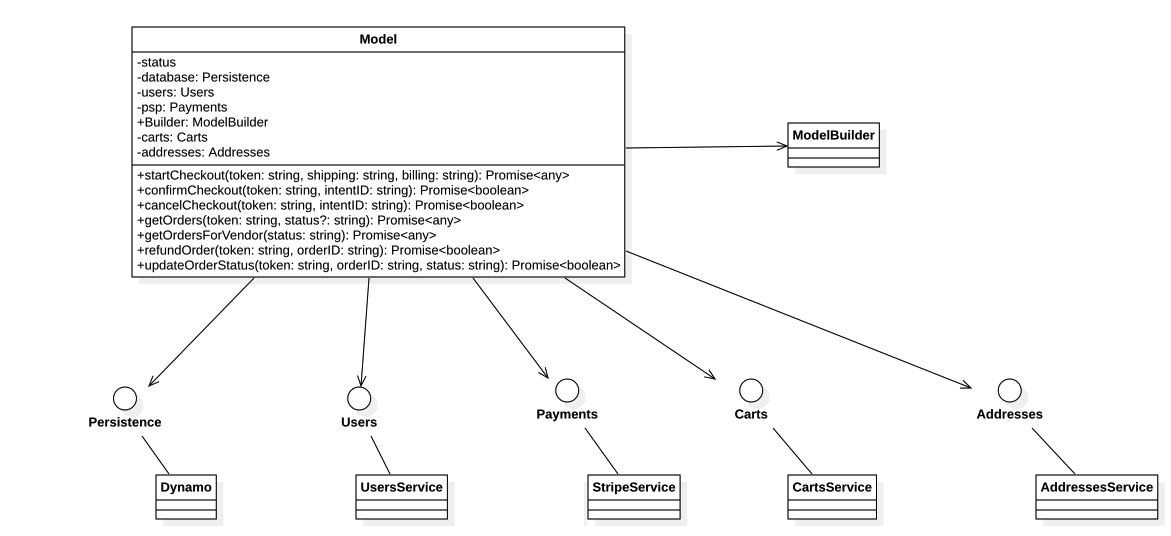
\includegraphics[width=\textwidth]{res/images/class-diagrams/orders.png}
\end{figure}

\subsubsection{Carts service}
\begin{figure}[H]
    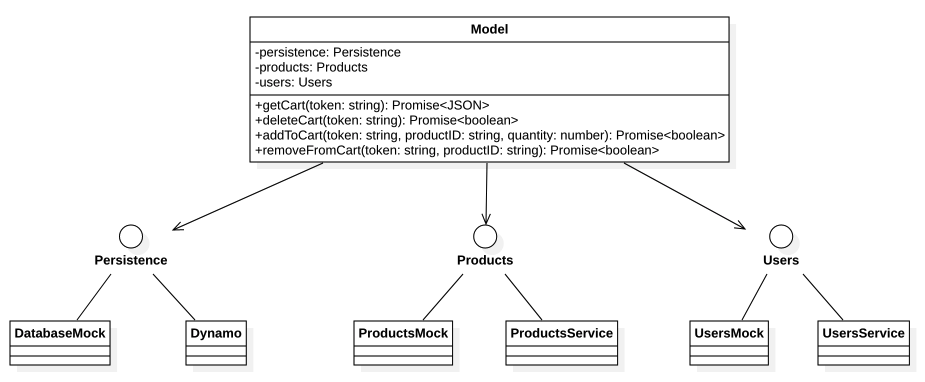
\includegraphics[width=0.9\textwidth]{res/images/class-diagrams/carts.png}
\end{figure}

\subsubsection{Addresses service}
\begin{figure}[H]
    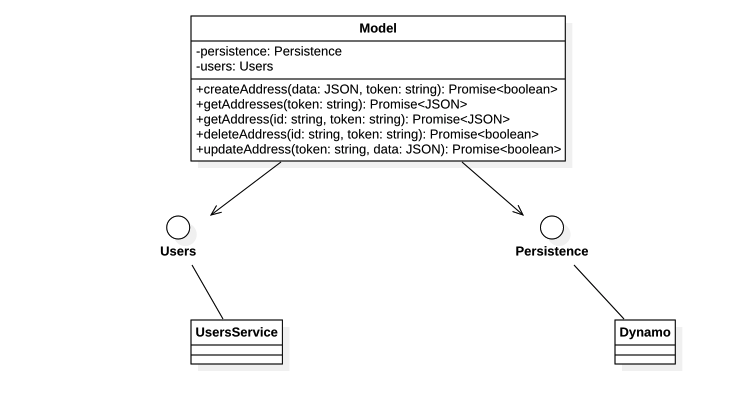
\includegraphics[width=0.9\textwidth]{res/images/class-diagrams/addresses.png}
\end{figure}

\subsubsection{Users service}
\begin{figure}[H]
    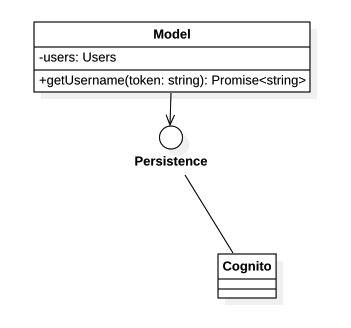
\includegraphics[width=0.45\textwidth]{res/images/class-diagrams/users.png}
\end{figure}

\subsection{Sequence diagrams}
In this section we'll provide sequence diagrams for explaining how microservices communicates between each others
when API's are called from the fronend service.

\subsubsection{Taxes service}
\begin{figure}[H]
    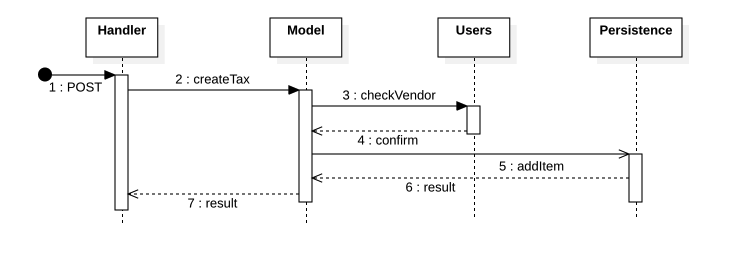
\includegraphics[width=0.9\textwidth]{res/images/sequence-diagrams/taxes/createTax.png}
\end{figure}

\begin{figure}[H]
    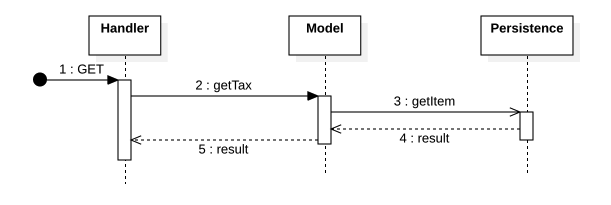
\includegraphics[width=0.9\textwidth]{res/images/sequence-diagrams/taxes/getTax.png}
\end{figure}

\begin{figure}[H]
    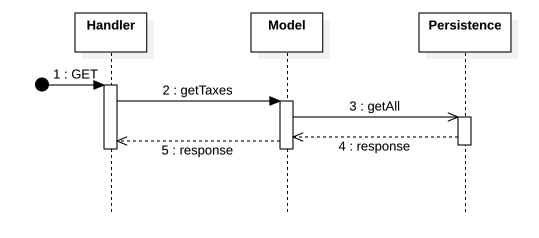
\includegraphics[width=0.8\textwidth]{res/images/sequence-diagrams/taxes/getTaxes.png}
\end{figure}

\begin{figure}[H]
    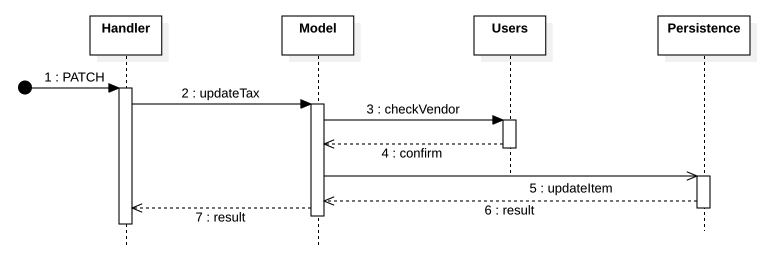
\includegraphics[width=0.8\textwidth]{res/images/sequence-diagrams/taxes/updateTax.png}
\end{figure}

\begin{figure}[H]
    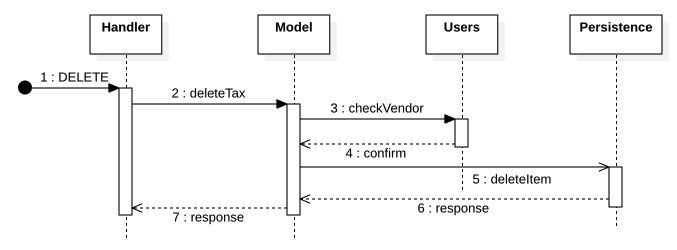
\includegraphics[width=0.9\textwidth]{res/images/sequence-diagrams/taxes/deleteTax.png}
\end{figure}

\subsubsection{Categories service}
\begin{figure}[H]
    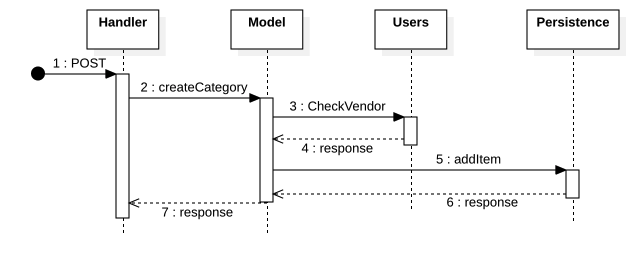
\includegraphics[width=0.9\textwidth]{res/images/sequence-diagrams/categories/createCategory.png}
\end{figure}

\begin{figure}[H]
    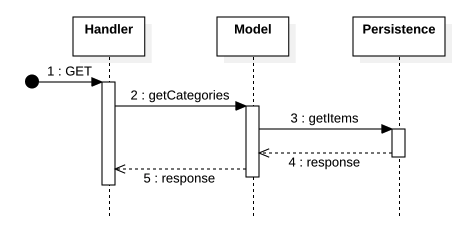
\includegraphics[width=0.8\textwidth]{res/images/sequence-diagrams/categories/getCategories.png}
\end{figure}

\begin{figure}[H]
    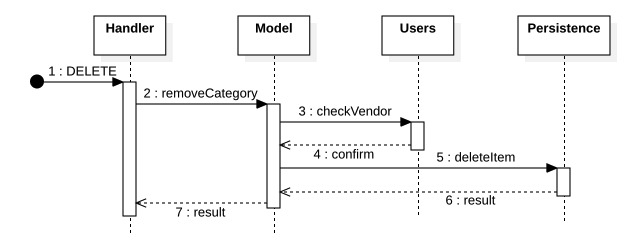
\includegraphics[width=0.9\textwidth]{res/images/sequence-diagrams/categories/removeCategory.png}
\end{figure}

\begin{figure}[H]
    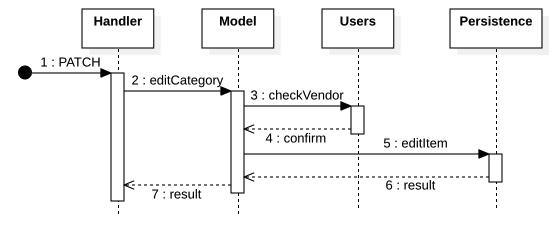
\includegraphics[width=0.9\textwidth]{res/images/sequence-diagrams/categories/updateCategory.png}
\end{figure}

\subsubsection{Orders service}
\begin{figure}[H]
    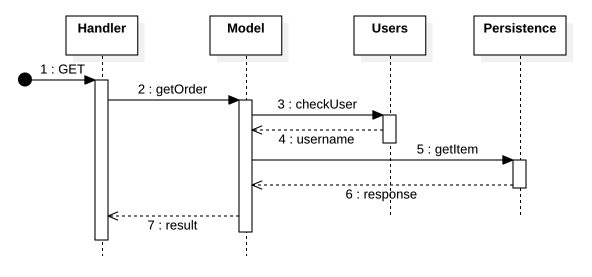
\includegraphics[width=0.9\textwidth]{res/images/sequence-diagrams/orders/getOrderByID.png}
\end{figure}

\begin{figure}[H]
    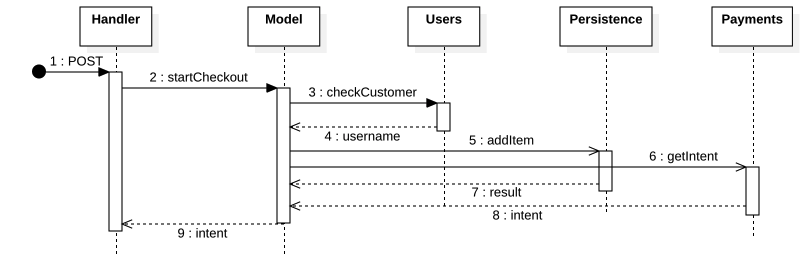
\includegraphics[width=0.9\textwidth]{res/images/sequence-diagrams/orders/startCheckout.png}
\end{figure}

\begin{figure}[H]
    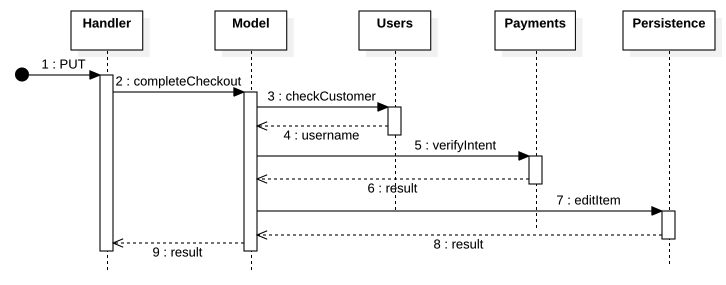
\includegraphics[width=0.9\textwidth]{res/images/sequence-diagrams/orders/completeCheckout.png}
\end{figure}

\begin{figure}[H]
    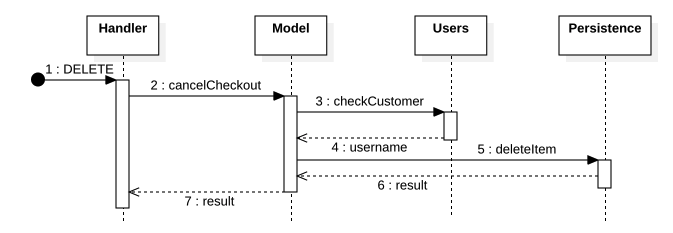
\includegraphics[width=0.9\textwidth]{res/images/sequence-diagrams/orders/cancelCheckout.png}
\end{figure}

\subsubsection{Carts service}

\begin{figure}[H]
    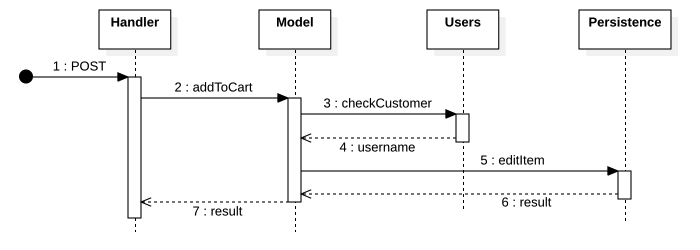
\includegraphics[width=0.9\textwidth]{res/images/sequence-diagrams/carts/addToCart.png}
\end{figure}

\begin{figure}[H]
    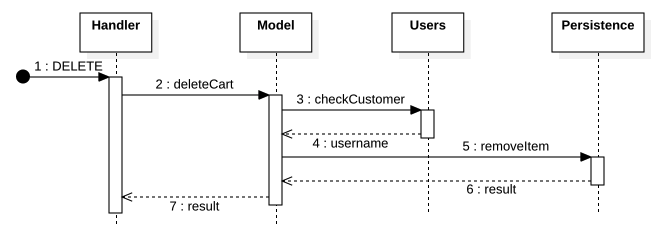
\includegraphics[width=0.9\textwidth]{res/images/sequence-diagrams/carts/deleteCart.png}
\end{figure}

\begin{figure}[H]
    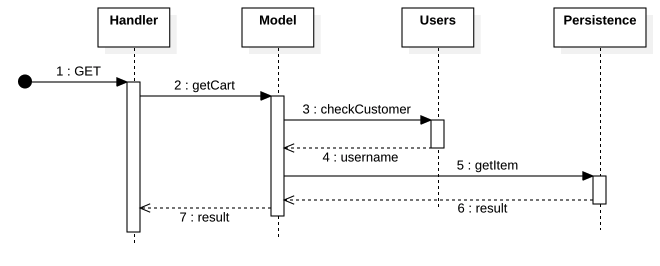
\includegraphics[width=0.9\textwidth]{res/images/sequence-diagrams/carts/getCart.png}
\end{figure}

\begin{figure}[H]
    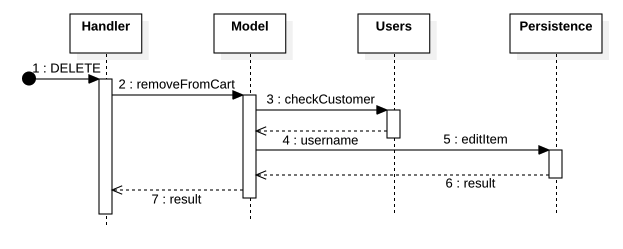
\includegraphics[width=0.9\textwidth]{res/images/sequence-diagrams/carts/removeFromCart.png}
\end{figure}

\subsubsection{Addresses service}

\begin{figure}[H]
    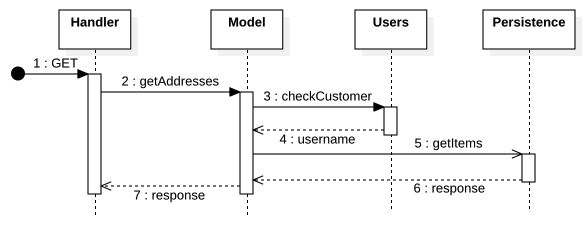
\includegraphics[width=0.9\textwidth]{res/images/sequence-diagrams/addresses/getAddresses.png}
\end{figure}

\begin{figure}[H]
    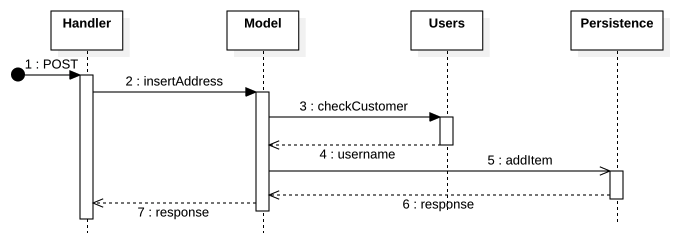
\includegraphics[width=0.9\textwidth]{res/images/sequence-diagrams/addresses/insertAddress.png}
\end{figure}

\begin{figure}[H]
    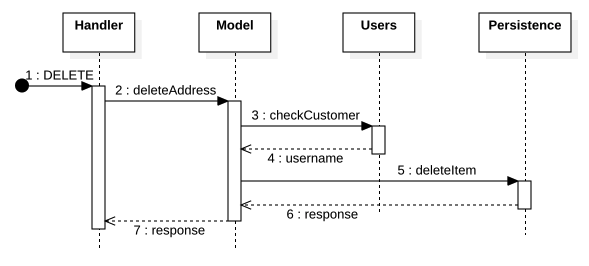
\includegraphics[width=0.9\textwidth]{res/images/sequence-diagrams/addresses/removeAddress.png}
\end{figure}

\begin{figure}[H]
    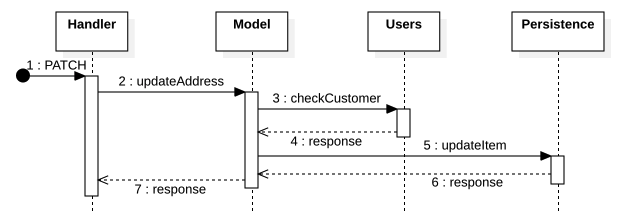
\includegraphics[width=0.9\textwidth]{res/images/sequence-diagrams/addresses/updateAddress.png}
\end{figure}



\subsubsection{Users service}

